%%
%% This is file `sample-sigconf.tex',
%% generated with the docstrip utility.
%%
%% The original source files were:
%%
%% samples.dtx  (with options: `sigconf')
%% 
%% IMPORTANT NOTICE:
%% 
%% For the copyright see the source file.
%% 
%% Any modified versions of this file must be renamed
%% with new filenames distinct from sample-sigconf.tex.
%% 
%% For distribution of the original source see the terms
%% for copying and modification in the file samples.dtx.
%% 
%% This generated file may be distributed as long as the
%% original source files, as listed above, are part of the
%% same distribution. (The sources need not necessarily be
%% in the same archive or directory.)
%%
%% The first command in your LaTeX source must be the \documentclass command.@
\documentclass[sigconf,nonacm=true]{acmart}
\usepackage{listings}
\usepackage{booktabs}% More professional look of tables.
\usepackage{siunitx}% An awesome package for typesetting and manipulation numbers and units.
\usepackage{caption}% Better control over caption
\usepackage{lipsum}% Example text
\usepackage{xcolor}
\usepackage{adjustbox}
\usepackage{booktabs}

\lstset{
	basicstyle=\ttfamily,
	columns=fullflexible,
	frame=single,
	breaklines=true,
	postbreak=\mbox{\textcolor{red}{$\hookrightarrow$}\space},
}

\pagecolor{white}
\lstset{
basicstyle=\ttfamily,
frame=single
}
%%
%% \BibTeX command to typeset BibTeX logo in the docs
\AtBeginDocument{%
  \providecommand\BibTeX{{%
    \normalfont B\kern-0.5em{\scshape i\kern-0.25em b}\kern-0.8em\TeX}}}

%% Rights management information.  This information is sent to you
%% when you complete the rights form.  These commands have SAMPLE
%% values in them; it is your responsibility as an author to replace
%% the commands and values with those provided to you when you
%% complete the rights form.
\setcopyright{none}
%%\copyrightyear{2020}
%%\acmYear{2020}
%%\acmDOI{10.1145/1122445.1122456}

%% These commands are for a PROCEEDINGS abstract or paper.
%% \acmConference[Woodstock '18]{Woodstock '18: ACM Symposium on Neural
%%   Gaze Detection}{June 03--05, 2018}{Woodstock, NY}
%% \acmBooktitle{Woodstock '18: ACM Symposium on Neural Gaze Detection,
%%   June 03--05, 2018, Woodstock, NY}
%% \acmPrice{15.00}
%% \acmISBN{978-1-4503-XXXX-X/18/06}


%%
%% Submission ID.
%% Use this when submitting an article to a sponsored event. You'll
%% receive a unique submission ID from the organizers
%% of the event, and this ID should be used as the parameter to this command.
%%\acmSubmissionID{123-A56-BU3}

%%
%% The majority of ACM publications use numbered citations and
%% references.  The command \citestyle{authoryear} switches to the
%% "author year" style.
%%
%% If you are preparing content for an event
%% sponsored by ACM SIGGRAPH, you must use the "author year" style of
%% citations and references.
%% Uncommenting
%% the next command will enable that style.
%%\citestyle{acmauthoryear}

%%
%% end of the preamble, start of the body of the document source.
\begin{document}

%%
%% The "title" command has an optional parameter,
%% allowing the author to define a "short title" to be used in page headers.
\title{CE/CZ4041 Project: Dog Breed Identification (Kaggle)}

%%
%% The "author" command and its associated commands are used to define
%% the authors and their affiliations.
%% Of note is the shared affiliation of the first two authors, and the
%% "authornote" and "authornotemark" commands
%% used to denote shared contribution to the research.

\author{Cao Hai Nam}
\authornote{All authors contributed equally to this project.}
\affiliation{\institution{Nanyang Technological University}}
\email{HAINAM001@e.ntu.edu.sg}

\author{Harold Teng Ze Chie}
\authornotemark[1]
\affiliation{\institution{Nanyang Technological University}}
\email{HTENG001@e.ntu.edu.sg}

\author{Kok Zi Ming}
\authornotemark[1]
\affiliation{\institution{Nanyang Technological University}}
\email{KOKZ0003@e.ntu.edu.sg}

\author{Manish Dhanetwal}
\authornotemark[1]
\affiliation{\institution{Nanyang Technological University}}
\email{MANISH007@e.ntu.edu.sg}

\author{Pang Yu Shao}
\authornotemark[1]
\affiliation{\institution{Nanyang Technological University}}
\email{C170134@e.ntu.edu.sg}

%%
%% By default, the full list of authors will be used in the page
%% headers. Often, this list is too long, and will overlap
%% other information printed in the page headers. This command allows
%% the author to define a more concise list
%% of authors' names for this purpose.
%% \renewcommand{\shortauthors}{Trovato and Tobin, et al.}

%%
%% The abstract is a short summary of the work to be presented in the
%% article.
%%\begin{abstract}
%%  TODO:
%%\end{abstract}



%%
%% Keywords. The author(s) should pick words that accurately describe
%% the work being presented. Separate the keywords with commas.
%% \keywords{Deep Learning, NLP, Neural Networks}

%% A "teaser" image appears between the author and affiliation
%% information and the body of the document, and typically spans the
%% page.

%% \begin{teaserfigure}
%%   \includegraphics[width=\textwidth]{sampleteaser}
%%   \caption{Seattle Mariners at Spring Training, 2010.}
%%   \Description{Enjoying the baseball game from the third-base
%%   seats. Ichiro Suzuki preparing to bat.}
%%   \label{fig:teaser}
%% \end{teaserfigure}

%%
%% This command processes the author and affiliation and title
%% information and builds the first part of the formatted document.
\maketitle

\section{Introduction}
In this project, a Machine Learning model is implemented to solve the 
task of classifying a dog's breed based on an input image as part of 
a Kaggle competition, "\textbf{Dog Breed Identification}\footnote[1]{\url{https://www.kaggle.com/c/dog-breed-identification/overview}}".

Various methods are experimented and evaluated in order to obtain a final 
Implementation of a model which is able to predict the given test data with the 
lowest error and thus provide a higher score on the Kaggle competition's leaderboard.
\section{Dataset}
The dataset provided for this task is a canine subset of the ImageNet dataset \cite{ILSVRC15}. Each of the images
belong to one of 120 different classes (breeds).

\subsection{Class Distribution}
\label{section:classdistro}
The training set was analysed to determine the distribution of classes for the training samples, the distribution 
can be seen in Figure \ref{fig:classdistro}.
\begin{figure}[H]
	\centering
	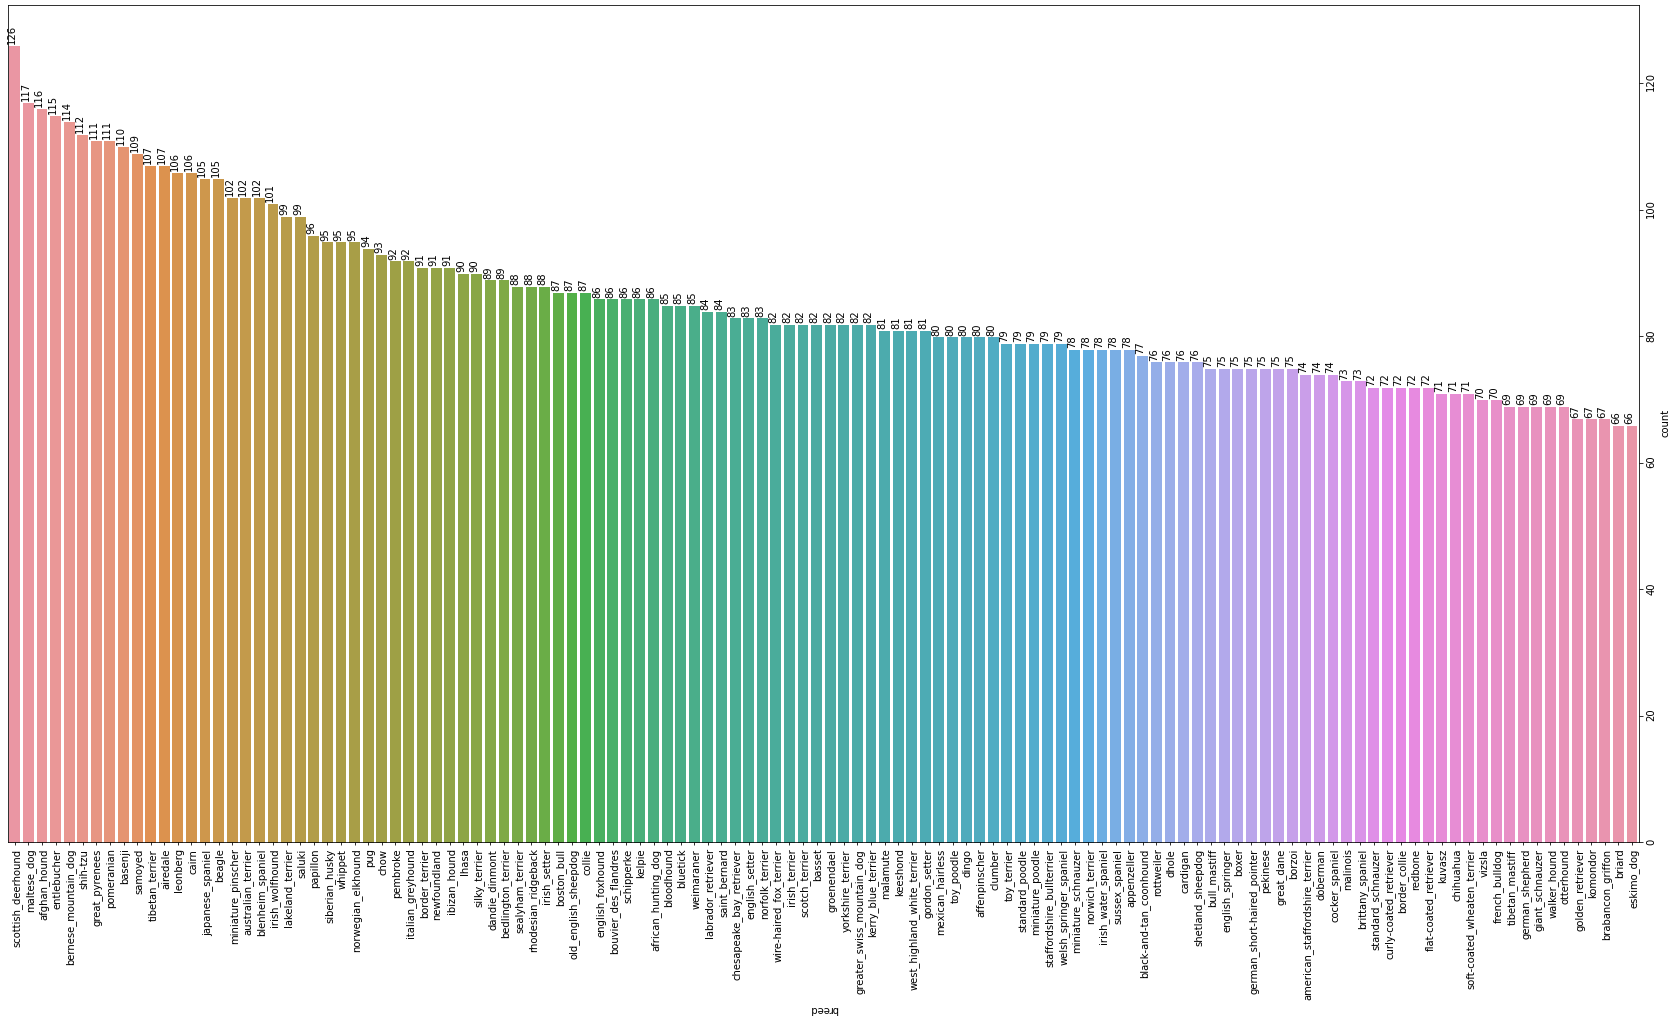
\includegraphics[width=0.9\linewidth]{fig/classdistribution.png}
	\caption{Distribution of Classes of Training Examples}
	\label{fig:classdistro}
\end{figure}
From Figure \ref{fig:classdistro}, it can be seen that the dataset is imbalanced. This may result in 
biases being learnt by the model during the training stage. Therefore, various strategies such as 
oversampling and undersampling will be explored to allow the model to make more accurate predictions
to unseen data.


\section{Implementation}
An Artificial Neural Network (ANN) was chosen for the implementation of the machine learning model with the use of 
\textbf{Transfer Learning} by using other pre-trained Deep Learning models for extracting learned features from the 
images. This extraction of features is done as a "preprocessing" step and is done before training time. The dataset 
is then rebuilt with the extracted features as the inputs while the output target label is unchanged.

A simple ANN is then implemented as the "classification head", which learns to classify the breed of the dog 
in the input image based on the extracted features. Since the dimension of feature vectors at the 
output of the pre-trained models are large, a dropout layer is also applied to prevent over-fitting by the ANN.
The architecture of the model is shown in Figure \ref{fig:tlarch}.

\begin{figure*}
	\centering
	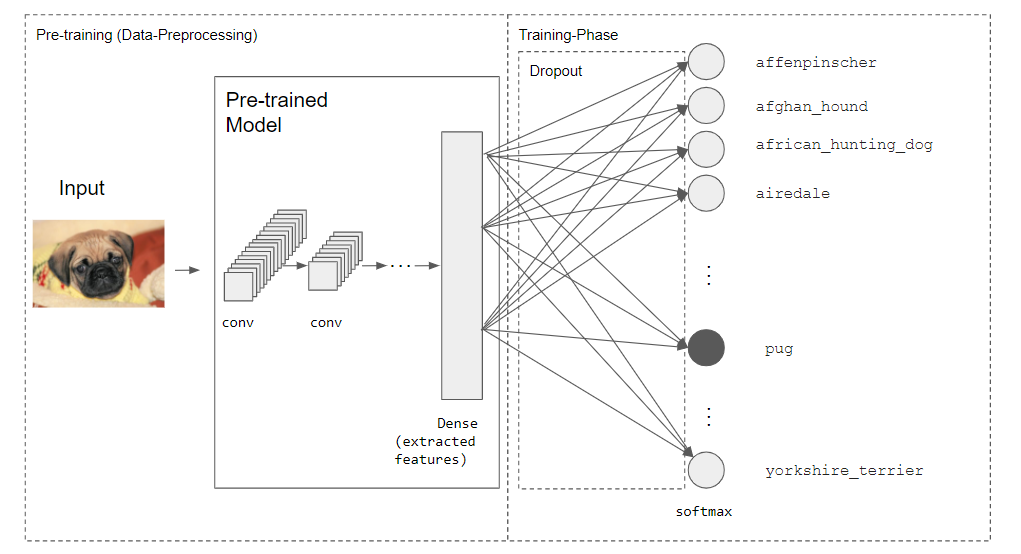
\includegraphics[width=0.9\linewidth]{fig/tlarch.png}
	\caption{Architecture of the ANN built on top of the pre-trained model}
	\label{fig:tlarch}
\end{figure*} 

\subsection{Transfer Learning}
Transfer Learning is defined as given a source domain and learning task and a target domain and learning task,
\textit{transfer learning} aims to improve the learning of the target predictive function in the target domain 
using the knowledge in the source domain and the source task, whereby the source task and domain is not the same 
as that of the target task and domain \cite{10.1109/TKDE.2009.191}.

With image datasets being publicly available such as ImageNet and COCO \cite{lin2015microsoft}, challenges 
such as the ImageNet Large Scale Visual Recognition Challenge (ILSVRC) as well as the COCO Challenge are 
held to spur research into tasks such as image classification or object detection. 

From these challenges, many State-of-the-Art neural network architectures have been published and made available,
such as: \textbf{Inception} \cite{43022} (ILSVRC2014) and \textbf{ResNet} \cite{he2015deep} (ILSVRC2015). Many other 
architectures are further built upon these existing architectures with improved performance, such as the 
\textbf{Inception-ResNet} \cite{szegedy2016inceptionv4} architecture, which is built upon both the Inception and ResNet
architectures.

As these pre-trained models are trained on the same dataset used in our task (i.e., ImageNet), the models' weights
are well-trained to extract high-level features from the images. Therefore, the pre-trained models can be adapted 
for use as feature extractors by removing the classification layer. The layer before the classification layer would 
thus provide an image vector when an image is fed into the input, which is essentially a representation of high-level 
features of the input image.

In this case, the source and target domains are the same while the source and target tasks are different. 
This is also known as \textit{Inductive transfer learning} which was introduced by Pan and Yang \cite{10.1109/TKDE.2009.191}.
Specifically, this is a case of \textit{Sequential transfer learning} (introduced by Ruder \cite{Ruder2019Neural}), where 
the tasks are learnt in sequence and the knowledge of the model trained on the source task is transferred to the target task.

\section{Experiment Results \& Model Selection}
In this section, experiments are carried out and evaluated to arrive at a final model which would give the highest score
which would be used to predict the classes of the unseen test data for submission to the Kaggle competition.

\subsection{Experimental Set-up}
\label{section:setup}
In each of the experiments carried out, the models will be evaluated based on the loss on the \textbf{validation set}.
The loss function would be the \textbf{multi-class log loss}, also known as the multi-class cross entropy. This loss function is also 
used in the judging of the submission by Kaggle. 

The optimiser used for training the model is the \textbf{Adam} optimiser, with learning rate annealing and early stopping 
applied when the validation loss is detected to not improve over a number of training cycles (\textbf{epochs}). Each of the 
models were trained until they were stopped by the early stopping mechanism.

\subsection{Pre-trained Model Selection}
\label{section:pretrainedmodels}
A few pre-trained models of varying architectures were used for feature extraction, and the extracted features
were used to train the ANN. The following pre-trained models were used as feature extractors in our experiments:

\begin{enumerate}
	\item InceptionV3 \cite{szegedy2015rethinking}
	\item Xception \cite{chollet2017xception}
	\item Inception-ResNetV2 \cite{szegedy2016inceptionv4}
	\item NASNetLarge \cite{zoph2018learning}
	\item BiT-S R101x3 \cite{kolesnikov2020big}
\end{enumerate}

Each of the models were evaluated by training the ANN with the same hyperparameters, with a learning rate of 
\textbf{0.0001}, and a drop probability of \textbf{50\%} with stratified k-fold cross-validation.
The following table shows the average validation loss from the model using each of the various 
pre-trained models as feature extractors:

\begin{table}[H]
	\begin{tabular}{cc}
		\toprule
		Feature Extractor&Average Loss (Cross-Entropy)\\
		\midrule
		InceptionV3 & 0.2614\\
		Xception & 0.2577\\
		Inception-ResnetV2 & 0.2361\\
		NASNetLarge & 0.2018\\
		BiT-S R101x3 & 0.2777\\
		\bottomrule
	\end{tabular}
	\caption{Comparison of performance from utilising Feature Extractors}
	\label{tab:featperf}
\end{table}

From Table \ref{tab:featperf}, it can be seen that the features extracted by the NASNetLarge model yielded the 
best performance when used as the inputs to our ANN. 


\subsection{Combining Features from Different Feature Extractors}
In an attempt to further increase the performance of the model, we experimented the concatenation of all features
obtained from \textbf{all} pre-trained models stated in Section \ref{section:pretrainedmodels}. This architecture is depicted
in Figure \ref{fig:finalarch}. With the new concatenated features, the ANN was trained with the same hyperparameters as the 
models trained from Section \ref{section:pretrainedmodels} and yielded a final average validation loss
of \textbf{0.17} as shown in Table \ref{tab:featperf2} below.

\begin{figure*}
	\centering
	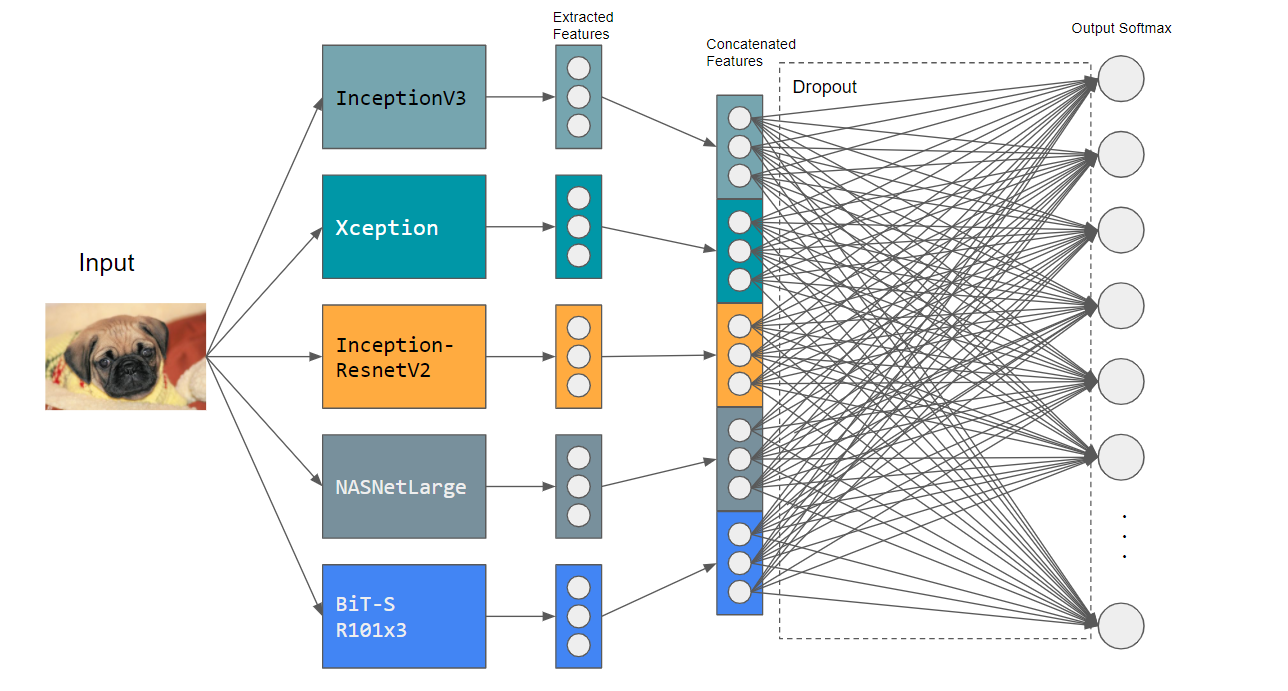
\includegraphics[width=0.95\linewidth]{fig/finalarch.png}
	\caption{Architecture of the ANN built on top of the concatenated features}
	\label{fig:finalarch}
\end{figure*} 


\begin{table}[H]
	\begin{tabular}{cc}
		\toprule
		Feature Extractor&Average Loss (Cross-Entropy)\\
		\midrule
		NASNetLarge (Best)& 0.2018\\
		Concatenated & 0.1752\\
		\bottomrule
	\end{tabular}
	\caption{Comparison of performance from utilising Feature Extractors}
	\label{tab:featperf2}
\end{table}
Therefore, the concatenated features will be used as inputs to our ANN as it yielded the 
best performance during our experiments.


\subsection{Hyperparameters Tuning}
With the feature extraction method decided, the next step for improving the performance of the model is to tune the 
hyperparameters used for the training of the model (i.e., \textbf{dropout} and \textbf{learning rate}). To accomplish this,
\textbf{Grid Search} was performed. Grid search is performed by trying out all combinations of the parameters and to compare 
the performance of the models trained with the combination of the hyperparameters chosen. Stratified k-fold cross-validation was 
performed for each of the combination to obtain the average loss of the model trained with the combination of hyperparameters.

\subsubsection{First Pass}
For the first pass, the grid search was performed with the following variable values:\\\\
$lr \in [0.0001, 0.0002, 0.0003, 0.0004,  0.0005]$\\
$dropout \in [0.1, 0.2, 0.3, 0.4,  0.5, 0.6, 0.7, 0.8, 0.9]$\\\\

After performing the grid search, the average validation loss of the model was recorded and plotted 
on a heatmap in Figure \ref{fig:gridsearch1} below:

\begin{figure}[H]
	\centering
	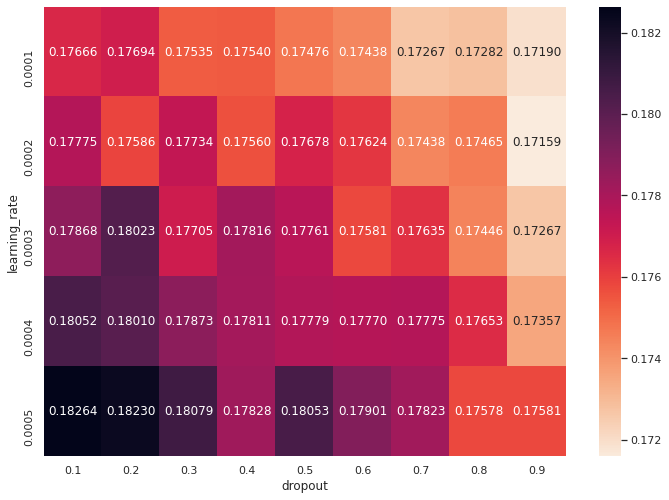
\includegraphics[width=\linewidth]{fig/gridsearch1.png}
	\caption{Results of Grid Search (First Pass)}
	\label{fig:gridsearch1}
\end{figure}

From the results, it can be seen that the model trained with a learning rate of \textbf{0.0002} and 
a dropout rate of \textbf{0.9} achieved the highest performance by having the lowest average
validation loss of \textbf{0.1716}.

\subsubsection{Second Pass}
The grid search was then repeated using a smaller resolution of values around the values obtained in the first pass 
of the grid search:\\\\
$lr \in [0.000125, 0.00015, 0.000175, 0.0002, 0.000225]$\\
$dropout \in [0.86, 0.88, 0.90, 0.92, 0.94, 0.96]$\\\\

After performing the grid search, the average validation loss of the model was recorded and plotted 
on a heatmap in Figure \ref{fig:gridsearch2} below:

\begin{figure}[H]
	\centering
	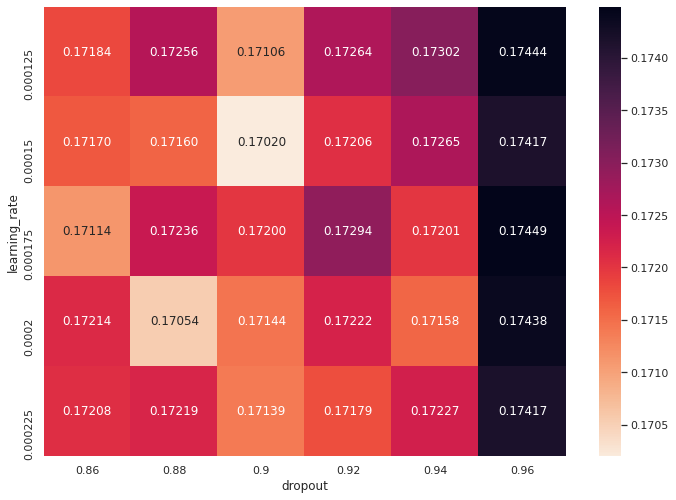
\includegraphics[width=\linewidth]{fig/gridsearch2.png}
	\caption{Results of Grid Search (Second Pass)}
	\label{fig:gridsearch2}
\end{figure}

From the results, it can be seen that the model trained with a learning rate of \textbf{0.00015} and 
a dropout rate of \textbf{0.9} achieved the highest performance by having the lowest average
validation loss of \textbf{0.1702}. These hyperparameters are thus selected for use for the rest of the
experiments.

\subsection{Overcoming Imbalanced Classes}
\label{section:imbaclass}
From Section \ref{section:classdistro}, we have identified that the dataset is slightly imbalanced where
some classes have more training examples than others. While the imbalance is quite small as compared to 
other classification tasks / datasets (e.g., credit card fraud detection), we experiment various strategies 
used for classification on imbalanced data to determine if they are effective in improving the performance 
of our model.

\subsubsection{Class Weights}
\label{section:classweights}
A simple way of overcoming the problem of imbalanced classes is to use "\textit{class weights}", which is 
to give a weighting for each class. The under-represented classes would have a higher weight and vice-versa.
This information is then fed to the model during training which will cause the model to "focus" more on the 
examples from the under-represented classes. The class weights can be calculated using the following formula:
\begin{displaymath}
	w_c = \frac{n\_samples}{n\_classes * n\_samples_c}
\end{displaymath}
This can be easily done without having to modify the training set by adding or removing training examples.

\subsubsection{Random Under/Oversampling}
The training dataset can also be balanced by performing Random Undersampling, where the over-represented 
training examples are removed at random such that there is an equal amount of training examples of each class.
While the training examples would be balanced, valuable training information may be lost in this process.
Similarly, Random Oversampling can also be performed on the training dataset to re-sample the under-represented
training examples with replacement such that the number of training examples are the same.

\subsubsection{Edited Nearest Neighbour Undersampling}
The Edited Nearest Neighbours (ENN) is an approach of resampling proposed by Wilson \cite{4309137} 
which aims to remove the majority class examples that are near the decision boundary. This is done by 
performing k-nearest neighbours classification on the examples of the majority classes and removing those 
that are misclassified as part of the minority class.

\subsubsection{Synthetic Minority Over-sampling Technique (SMOTE)}
SMOTE is an approach of generating synthetic training examples of the minority classes proposed by 
Chawla, Bowyer, Hall, \& Kegelmeyer \cite{Chawla_2002}. The synthetic training exmaples are generated by 
joining a minority example to \textit{k} neighbours belonging to the same class with a straight line 
and generating the synthetic examples along those lines.

\subsubsection{SMOTEENN}
\label{section:smoteenn}
SMOTEENN is a resampling strategy proposed by Batista, Prati and Monard \cite{10.1145/1007730.1007735}, 
which is essentially combination of SMOTE and ENN by first performing SMOTE then using ENN for data cleaning
to produce better clusters of class examples.

\subsubsection{Performance Evaluation}. The strategies mentioned in Section \ref{section:classweights} to 
\ref{section:smoteenn} were implemented and trained with the model with the holdout cross-validation. This is such that 
the resampling strategies would be applied to the same training examples and the models trained would be evaluated with 
the same validation set. The validation losses and prediction accuracy were obtained
and the performance of the models are shown in the table below:

\begin{table}[H]
	\begin{adjustbox}{width=\columnwidth}
	\begin{tabular}{rcc}
		\toprule
		Strategy&Average Loss (Cross-Entropy)&Prediction Accuracy\\
		\midrule
		Base Model & 0.1620 & 95.0\%\\
		\textbf{Class Weights} & \textbf{0.1608} & \textbf{95.2\%}\\
		Random Undersampling & 0.1690 & 94.8\%\\
		ENN & 0.2075 & 94.0\%\\
		Random Oversampling & 0.1627 & 94.9\%\\
		SMOTE & 0.1612 & 94.9\%\\
		SMOTEENN & 0.1776 & 94.7\%\\
		\bottomrule
	\end{tabular}
	\end{adjustbox}
	\caption{Comparison of performance of models trained from different resampling/ class weights}
	\label{tab:sampperf}
\end{table}
From Table \ref{tab:sampperf}, it can be seen that by applying information about the class weights 
to the model for training, the trained model yielded the best performance as compared to the other 
resampling technique and the baseline model. Therefore, this strategy is implemented in favour of other 
resampling strategies for the implementation of our final model.

\subsection{Model Selection}
\label{section:modelselection}
With the results obtained from performing the experiments conducted in Sections \ref{section:setup} - 
\ref{section:imbaclass}, the final model implemented for our task is the following:\\

\begin{itemize}
	\item Feature Extractors: Concatenated features from pre-trained models (InceptionV3, Xception, Inception-ResNetV2, NASNetLarge, BiT-S R101x3)
	\item Dropout drop probability: 0.9
	\item Learning Rate: 0.00015 (with annealing)
	\item Optimiser: Adam
	\item Loss function: Multi-class log loss
	\item Training Epochs: 500 (With early termination)
	\item Class distribution information fed to model during training (Class Weights)
\end{itemize}

\section{Kaggle Evaluation Score and Rank}
\subsection{Evaluation Score}
The model chosen in Section \ref{section:modelselection} was trained with the training dataset with holdout cross-validation
(70\% train, 30\% validation) and the model was used to predict the breeds of the dog images in the test set provided by the 
Kaggle competition. The predictions of the test images are output to a .csv file and was uploaded to Kaggle for evalation and 
the score that was obtained was \textbf{0.16846}.


\begin{figure}[H]
	\centering
	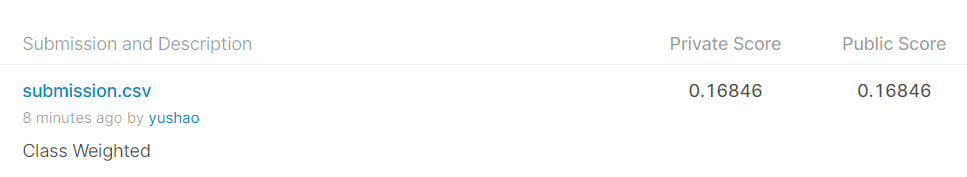
\includegraphics[width=\linewidth]{fig/submissionscore1.PNG}
	\caption{Kaggle Evaluation Score}
	\label{fig:eval1}
\end{figure}

\subsection{Evaluation Rank}
With the score of 0.16846, our model's performance was ranked 182nd in the Kaggle competition's 
leaderboard out of 1281 particiants, therefore our submission is within the \textbf{top 15\%} of the submissions 
for this competition.
\begin{figure}[H]
	\centering
	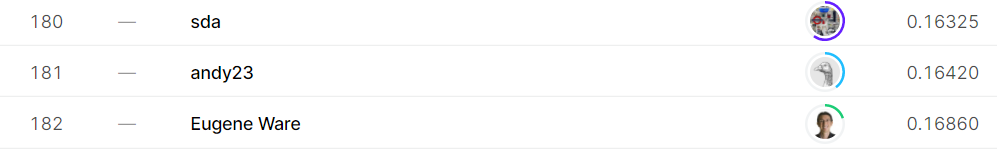
\includegraphics[width=\linewidth]{fig/lb1.PNG}
	\caption{Kaggle Leaderboard Position}
	\label{fig:lb1}
\end{figure}


\section{Conclusion}
In this project, we have successfully implemented a classifier for predicting the breed of a dog given a photo for the 
Kaggle competition. We have also managed to learn about Transfer Learning and have successfully applied it by utilising 
State-of-the-Art pre-trained models for feature extraction and further improved the performance of our model by 
tuning the hyperparameters used for the training of the model. 

We have also managed research and learn about the different techniques used when performing classification on an imbalanced
dataset and applied it to further improve the model's performance.

As a result, our implemented model was able to achieve top 15\% in the competition's leaderboard.



\bibliographystyle{ACM-Reference-Format}
\bibliography{bibfile}


\end{document}
\endinput
%%
%% End of file `sample-sigconf.tex'.
